Quantifying the uncertainty of neural networks' (NNs) predictions is important in safety-critical applications such as medical-diagnosis \cite{UIinMedicine} and self-driving vehicles \cite{McAllister2017ConcretePF,AutoDrivingBayes}.
Architectures for classification tasks produce a probability distribution as their output, constructed by applying the softmax to the point-estimate output of the penultimate layer.
However, it has been shown that this distribution is overconfident \citep{nguyen2015deep,Hein_2019_CVPR} and thus cannot be used for predictive uncertainty quantification.

Approximate Bayesian methods provide quantified uncertainty over the network's parameters and thus the outputs in a tractable fashion. The commonly used Gaussian approximate posterior \citep{MacKay1992,Graves2011VB,Blundell2015WeightUI,ritter2018a} approximately induces a Gaussian distribution over the logits of a NN \citep{McKay1995NetworkBayesReview}. However, the associated predictive distribution, which is the expectation of the softmax function w.r.t. the Gaussian, does not have an analytic form.
It is thus generally approximated by Monte Carlo (MC) integration requiring multiple samples. Predictions in Bayesian neural networks (BNNs) are thus generally expensive operations.

\begin{figure}[htb]
     \centering
     \subfloat{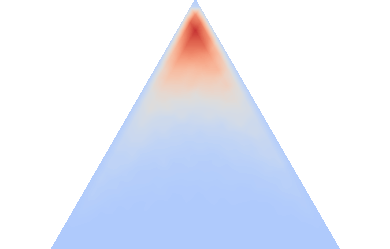
\includegraphics[width=0.4\textwidth]{figures/sMAP/sMAP_Gaussian_coolwarm_0.png}}
     \subfloat{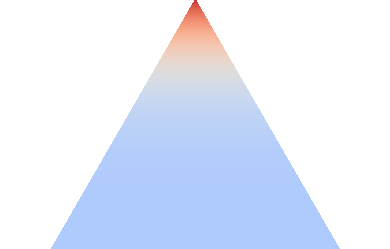
\includegraphics[width=0.4\textwidth]{figures/sMAP/sMAP_Dirichlet_coolwarm_0.png}}

    \setcounter{subfigure}{0}

     \subfloat[Monte Carlo]{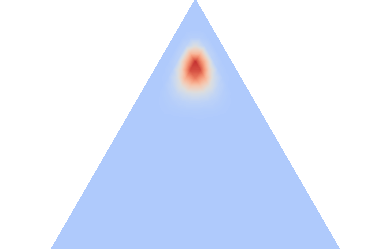
\includegraphics[width=0.4\textwidth]{figures/sMAP/sMAP_Gaussian_coolwarm_1.png}}
     \subfloat[Laplace Bridge]{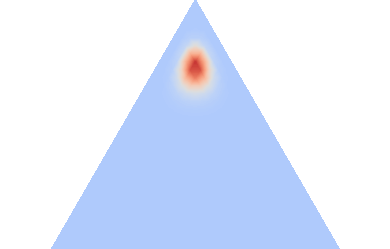
\includegraphics[width=0.4\textwidth]{figures/sMAP/sMAP_Dirichlet_coolwarm_1.png}} \\
     \caption{Densities on the simplex of the true distribution (left column, computed by exhaustive sampling by mapping a Gaussian random variable through the softmax transformation) and ``Laplace Bridge'' approximation constructed in this thesis (right column). For the top and bottom rows, two different Gaussians were used, such that the resulting mode is the same, but the uncertainty differs.}
    \label{fig:LPbridge_sMAP}
\end{figure}
	
In this thesis, we re-introduce an old but largely overlooked idea originally proposed by David JC \citet{MacKay1998} in a different setting (arguably the inverse of the Deep Learning setting). Dirichlet distributions are generally defined on the simplex. But when its variable is defined on the inverse softmax's domain, its shape effectively approximates a Gaussian. The inverse of this approximation, which will be called the \emph{Laplace Bridge} here \citep{KernelTopicModels2012}, analytically maps a Gaussian distribution onto a Dirichlet distribution. Given a Gaussian distribution over the logits of a NN, one can thus efficiently obtain an approximate Dirichlet distribution over the softmax outputs (\Cref{fig:LPbridge_sMAP}). Our contributions in this thesis are: We re-visit MacKay's derivation with particular attention to a symmetry constraint that becomes necessary in our ``inverted'' use of the argument from the Gaussian to the Dirichlet family. We then validate the quality of this approximation both by theoretical and empirical arguments, and demonstrate significant speed-up over MC-integration. Finally, we show a use-case, leveraging the analytic properties of Dirichlet distributions to improve the popular top-$k$ metric through uncertainties.

We think that the Laplace Bridge is a valuable method to estimate predictive uncertainty because it is easy to add to already existing architectures and it is very fast compared to sampling schemes. When combined with a Laplace approximation of the weights, the Laplace Bridge can use pre-trained models and is, therefore, a simple extension to existing architectures. The cost of computing the Laplace Bridge are lower than drawing one (!) sample from a Gaussian distribution over the outputs and the result is a fully parameterized Dirichlet distribution over the output space. This implies that the computational cost during application is reduced to a minimum. Having fast predictive uncertainty is important because it means viability for safety-critical applications, e.g. self-driving cars where a difference of milliseconds can increase safety and be used in rapid succession for multiple hundred frames per second. 

\Cref{chap:background} provides the mathematical derivation. \Cref{chap:method} and \ref{sec:practicalities} discuss the Laplace Bridge in the context of neural networks and with a deeper analysis of different ways to do posterior inference. We compare it to the recent approximations of the predictive distributions of NNs in \Cref{chap:related_work}. Empirical experiments are presented in \Cref{chap:experiments}.
